\documentclass[journal]{IEEEtran}
\IEEEoverridecommandlockouts
\usepackage{cite}
\usepackage[cmex10]{amsmath}
\usepackage{graphicx}
\usepackage{graphics}
\usepackage{subfigure}
\usepackage{epsfig}
\usepackage{algorithmic}
\usepackage[linesnumbered,ruled,slide]{algorithm2e}
\usepackage{amsfonts}
\usepackage{float}
\usepackage{enumerate}
\usepackage{verbatim}
\usepackage{caption3}
\usepackage{bm} %%公式加粗
\usepackage[justification=centering]{caption}




\begin{document}


\title{A Linear Programming Approach to Sequence-Based Localization in Acoustic Sensor Networks}


\author{\IEEEauthorblockN{Naigao Jin, Xiangyu Zhao, Xiangqi Kong, Lei Wang}
\IEEEauthorblockA{School of Software, Dalian University of Technology, China\\
Key Laboratory for Ubiquitous Network and Service Software of Liaoning Province\\
Email: ngjin@dlut.edu.cn, lei.wang@ieee.org}
}

% make the title area
%\maketitle
%\thispagestyle{plain}
%\pagestyle{plain}
\maketitle
\thispagestyle{empty}
\pagestyle{empty}

\begin{abstract}
%\boldmath

Acoustic source localization in sensor network is a challenging task because of severe constraints on cost, energy, and effective range of sensor devices. 
To overcome these limitations in existing solutions, this paper formally describes, designs, implements, and evaluates a Linear Programming method to Sequence-Based Localization, i.e., LPSBL, in distributed smartphone networks. 
The localization space can be divided into distinct regions, and each region can be uniquely identified by the node sequence that represents the ranking of distances from the reference nodes to that region. 
The key idea behind LPSBL is to turn the localization problem into linear feasibility problem by processing the node sequence. 
The proposed design is evaluated through theoretical analysis, extensive simulations, and physical experiments (an indoor test-bed with 30 smartphone nodes). 
Evaluation results demonstrate that LPSBL can effectively localize the acoustic source with good robustness.

\end{abstract}

\begin{IEEEkeywords}
sequence-based localization, linear programming, wireless sensor networks
\end{IEEEkeywords}



\IEEEpeerreviewmaketitle

\section{Introduction}

Acoustic source localization (ASL) plays an important role in a wide range of application scenarios, such
as speaker-location-aware audio capturing in videoconferencing \cite{guo2011localising}, shooter localization in a battle field \cite{sallai2011acoustic}, and wild biological acoustic studies \cite{allen2008voxnet}. 
The traditional centralized microphone array-based solution to ASL exploited multiple synchronized microphones to simultaneously acquire multiple signals, 
which have some limitations with regard to the distances between the microphones, and sensing range for the large-scale applications.
Wireless acoustic sensor networks (WASNs) can overcome these limitations. 
A WASN consists of a set of wireless microphone nodes that are spatially distributed over the environment, usually in an ad-hoc fashion. 
Due to the wireless communication capabilities, the array-size limitations disappear and the microphone nodes can physically cover a much larger area. 

Acoustic source localization problem in sensor networks has been widely studied in the literature. 
ASL in WASN is becoming feasible due to recent advances in personal portable computing devices with the rapid deployment ability.
% Wang, \emph{et al.} \cite{wang2003acoustic} described a system having static cluster architecture, the system experienced a problem in that the accuracy decreased when an acoustic source occurred between the clusters.
% Chen, \emph{et al.} \cite{chen2004dynamic} showed that nodes in the system did not need to recognize their cluster head, reducing the constraints on deployment of the localization system.
% Hu, et al. \cite{hu2009design} design the system based on 2-tier architecture, which experienced cost and deployment problems especially in the very large target area.
% Rabbat, \emph{et al.} \cite{rabbat2005robust} proposed a decentralized algorithm based on the distributed ML estimation technique using token ring architecture.
% Kim, \emph{et al.} \cite{kim2009locating} proposed to identify the node closest to the acoustic source, based on TOA comparisons between all nodes, thus incurring high communication cost and requiring global synchronization between all sensor nodes.
% Lightning is a method proposed in \cite{wang2008lightning} to identify the sensor closest to the acoustic source, also based on expensive broadcasting/flooding.
Most of the distributed acoustic source localization systems are range-based localization, which are built on top of distance or angle measurements among sensor nodes. 
These approaches can provide good localization performance, however, generally require costly hardware and have limited effective range due to energy constraints. 
The requirement of low cost and power prohibits many range-based methods for sensor node localization, especially for large-scale deployments. 
Yedavalli, \emph{et al.}~\cite{yedavalli2008sequence} proposed a Sequence-Based Localization (SBL) in wireless sensor networks. The heart of SBL is the division of a 2D localization space into distinct regions by the perpendicular bisectors of lines joining pairs of reference nodes (nodes with known locations).
Each distinct region formed in this manner can be uniquely identified by a location sequence that represents the distance ranks of reference nodes to that region. 
The unknown node first determines its own location sequence based on the measurement between itself and the reference nodes, then searches through the location sequence table to determine its location.

In this paper, we present a Linear Programming method to Sequence-Based Localization (LPSBL) by processing the node sequence. 
As a range-free approach, this design applies node sequences instead of direct distance
or TOA measurements for localization, and brings in the following two advantages: (i) node sequences feature better
robustness to the measurement noise; (ii) node sequences significantly alleviate the accuracy requirement of network level time synchronization. 
Compared with earlier works on sequence-based localization in sensor
networks (e.g. SBL~\cite{yedavalli2008sequence}), the primary contribution
of this article is providing an effective and optimal approach
to solve the sequence-based localization problem for sensor networks. 
Without brute-force searching in SBL, the proposed LPSBL system formulates the
sensor node localization as an convex optimization problem
of finding a feasible solution to a system of multiple linear
inequalities, which is produced by the node sequences.
Then, linear programming (LP) can be applied to reliably
and efficiently deal with the convex optimization problem,
even in large-scale sensor networks. The proposed design
is evaluated with both test-bed experiments and extensive
simulations. Evaluation results show that the proposed
LPSBL system can provide improved node localization
accuracy.


The rest of the article is organized as follows. Section \uppercase\expandafter{\romannumeral 2} presents an overview of the  localization system.
Then, the LPSBL is introduced in section \uppercase\expandafter{\romannumeral 3}.
Section \uppercase\expandafter{\romannumeral 4} discusses several practical issues.
Section \uppercase\expandafter{\romannumeral 5} presents simulation results and an empirical evaluation. Section \uppercase\expandafter{\romannumeral 6} briefly surveys related work.
Section \uppercase\expandafter{\romannumeral 7} concludes the whole article.





\section{System Overview}

% ˫����ʽ�м��������ͼ��:��\begin{figure*}  \end{figure*} 
\begin{figure}[htb]
  \centering
 %\setlength{\abovecaptionskip}{-15pt}
 %\setlength{\belowcaptionskip}{-5pt}
    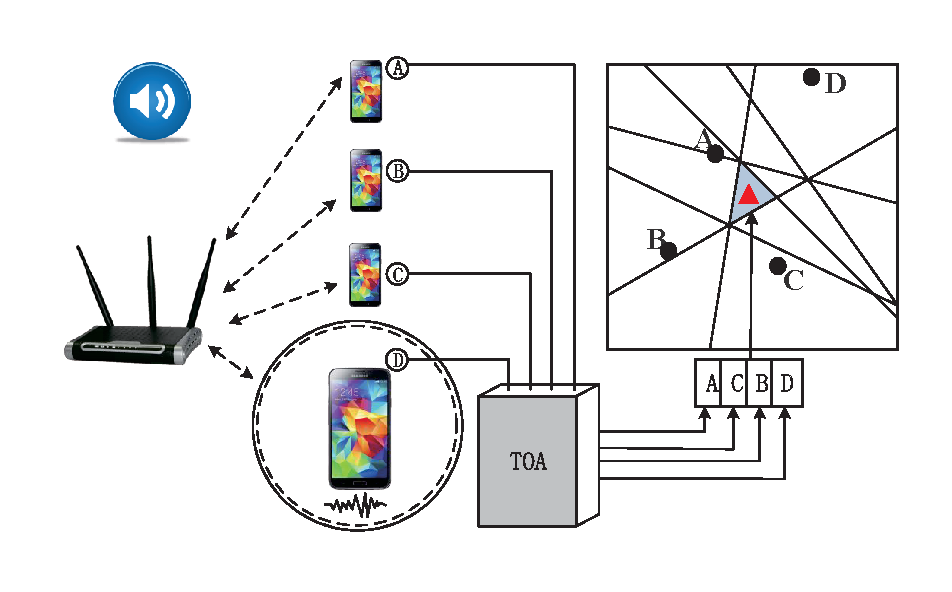
\includegraphics[height=4.5cm]{image/fig1.eps} 
    \caption{Overview of LPSBL}
 \label{overview}
    \end{figure}
\vspace{-5mm}

In this section, we focus mainly on the system overview of our LPSBL system, which aims at locating an unknown node. 
Fig. 1 shows a layout of a sensor network with anchor nodes and the acoustic source.
We use circles to denote anchor nodes with known locations and the triangle to denote the acoustic source.
Assume that a 2D localization space consists of
$N$ reference nodes. Consider any two reference nodes and
draw a perpendicular bisector to the line joining their
locations. This perpendicular bisector divides the localization
space into two different regions that are distinguished
by their proximity to either reference nodes, as illustrated in
Fig. 1. Similarly, if perpendicular bisectors are drawn for
all pairs of reference nodes, they divide the localization
space into many regions.
All locations inside a region have the same location
sequence. If each region in the arrangement is represented by
its centroid, then there is a one-to-one mapping relationship
between a location sequence and the centroid of the corresponding region that it represents.

Briefly, sequence-based localization system works as follows. 
After the acoustic source generates a sound, anchor nodes detect the event sequentially at different time instances that naturally gives an ordering of related nodes, called a node sequence. 
For instance, in Fig. 1, when the acoustic source generates a wave, the node sequence $NodeSeq (A C B D)$ is obtained along the sound propagation. 
The location information of acoustic source is embedded within the node sequence. 
The node sequence of a given region is unique to that region.
By collecting all sensing results, locations of the acoustic source can be estimated by processing the node sequence. 

Specifically, as shown in Fig. 2, $NodeSeq (A C B D)$ can be obtained by time of arrival (TOA) information of the acoustic event.
Moreover, the TOA sequence ${t_A} < {t_C} < {t_B} < {t_D}$ is determined by the distance sequence ${d_A} < {d_C} < {d_B} < {d_D}$ from each node to the acoustic source $S$.

\noindent \textbf{Problem 1:} Assume that the location of acoustic source is known, the node sequence can be obtained by the distances from nodes to the acoustic source.

Sequence-based localization is the inverse problem of Problem 1, can be described as follows.

\noindent \textbf{Problem 2:} Assume that the node sequence obtained from the TOA measurement is known, estimate the location of an acoustic source.

    \begin{figure}[!htb]
    \centering
 \setlength{\abovecaptionskip}{-15pt}
                     \vspace{-5mm}  
 %\setlength{\belowcaptionskip}{-5pt}
    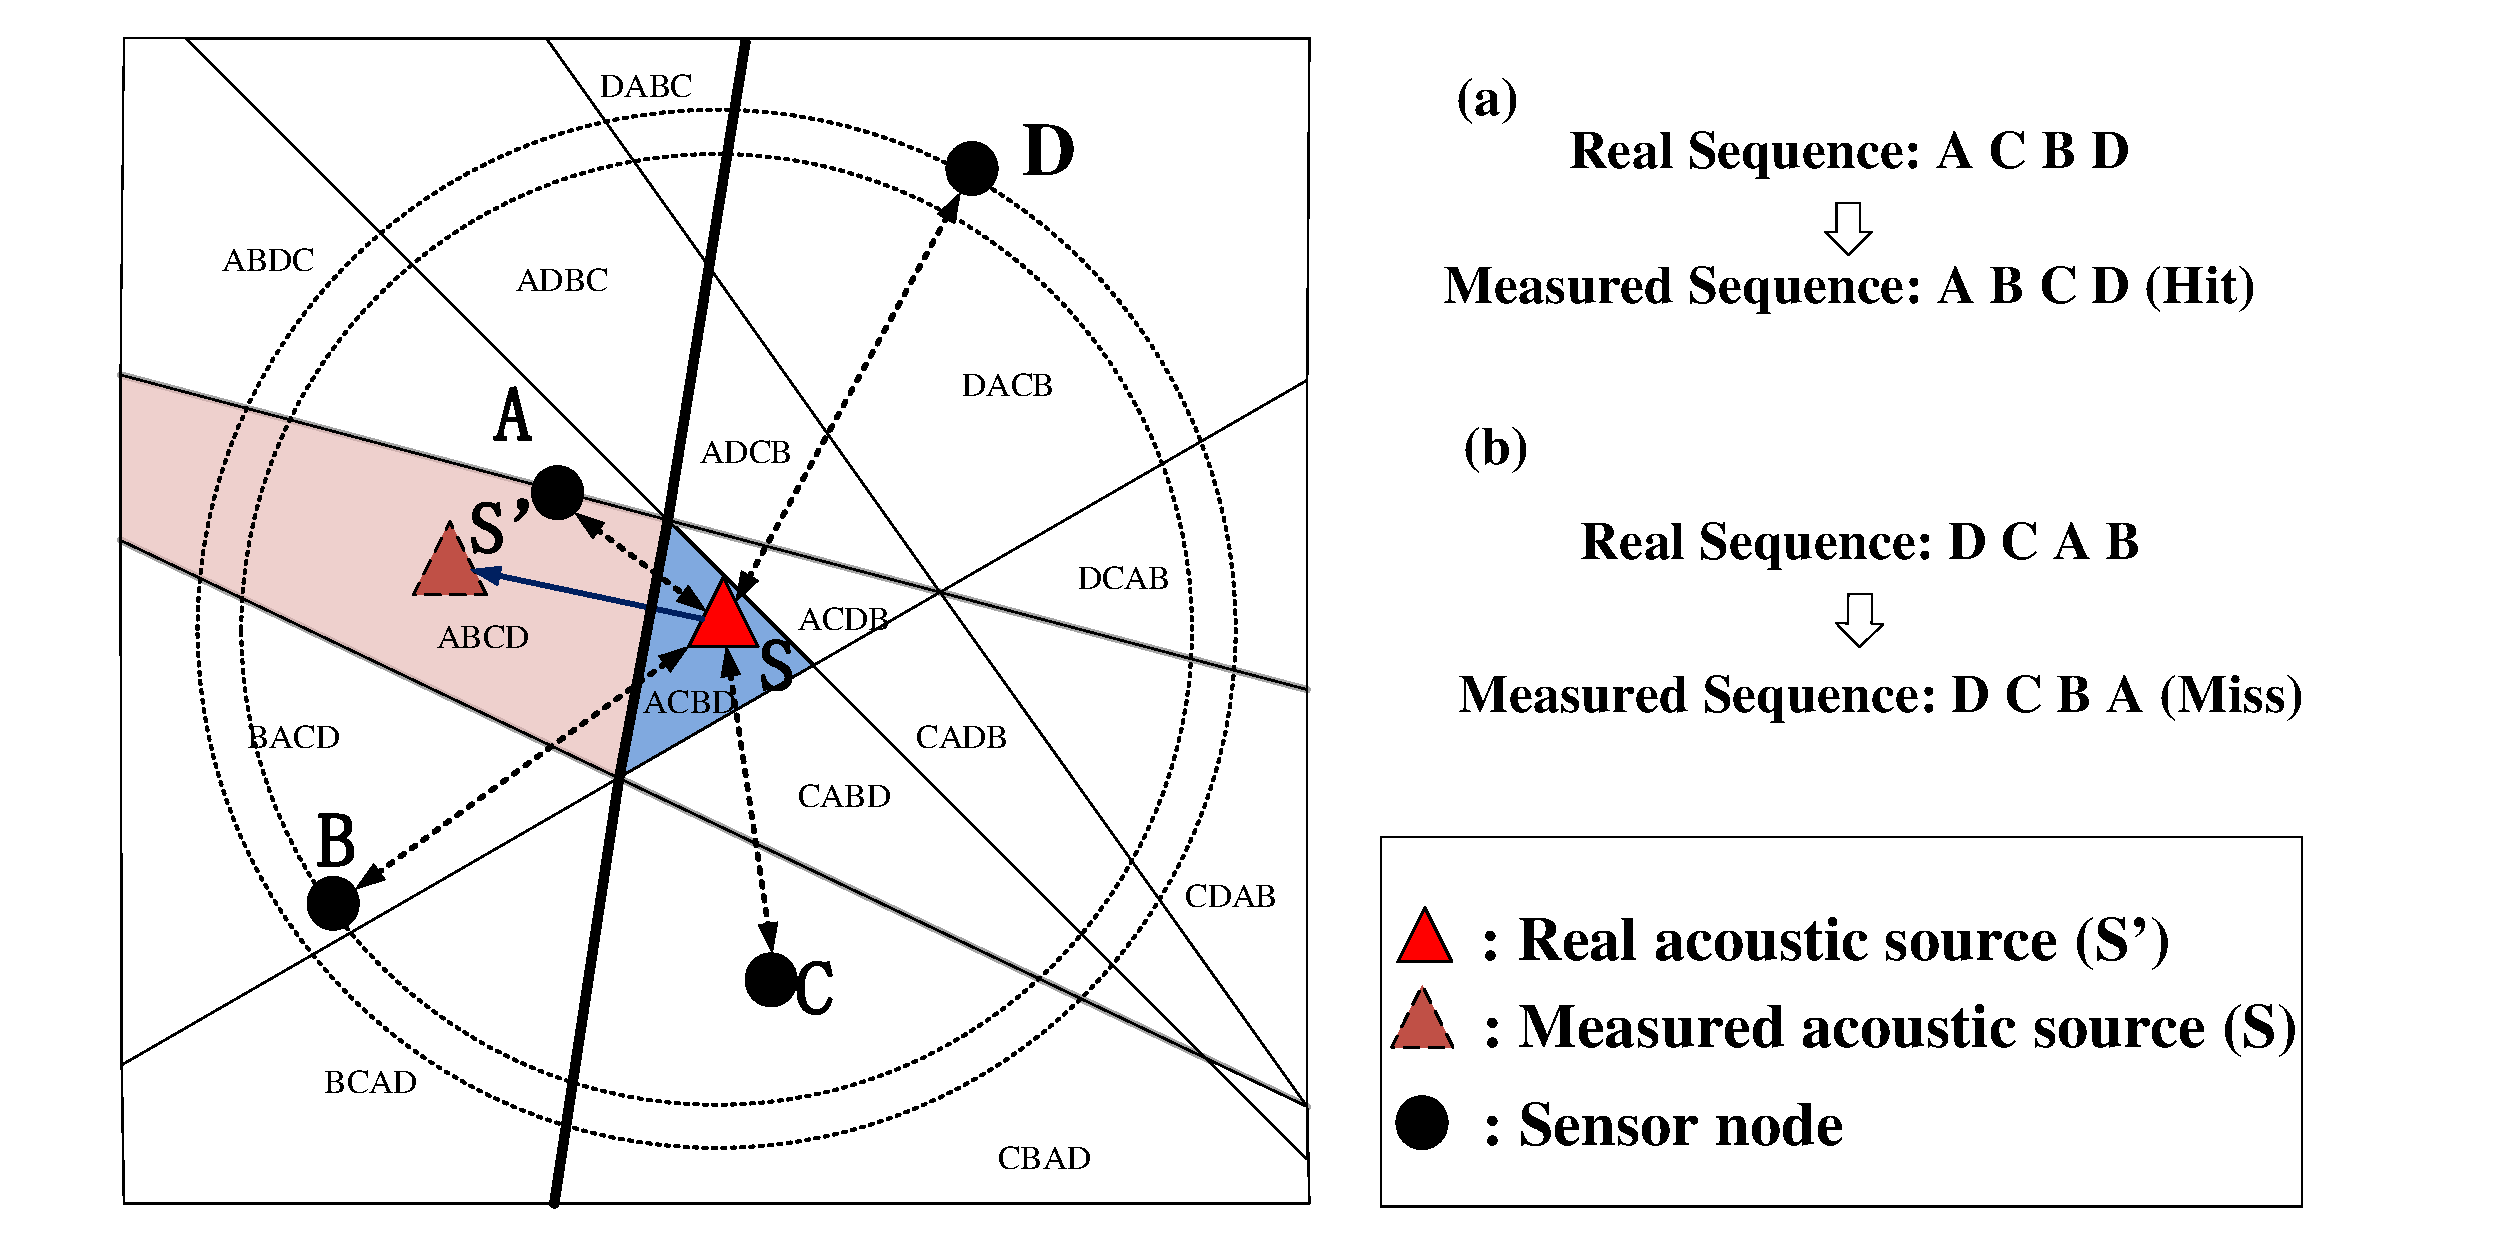
\includegraphics[height=4.5cm]{image/fig2.eps} 
	\vspace{10mm}
    \caption{The basic idea of LPSBL}
	\label{fig2}
    \vspace{-5mm}
    \end{figure}

In practice, solving the inverse problem is extremely difficult. 
In prior research, SBL estimated the location of nodes roughly by using a searching method with heavy computation. 
While in this paper, we carefully formulate Problem 2 as a convex optimization issue and propose an efficient solution which can provide the optimal localization results. 
To the best of our knowledge, this is the first work to leverage convex optimization for solving sequence-based localization problems in sensor networks.







\section{DESIGN}

In this section, we firstly introduce the basic LPSBL method.
After the basic LPSBL method is proposed, then we describe the robust LPSBL method in the next subsection.
Finally, the computational complexity analysis of LPSBL is given.

\subsection{Basic LPSBL}

In this section, we introduce the basic sequence-based localization technique based on linear programming method.

Considering a sensor network in the 2D space with $N$ nodes, all nodes is $\bm{X} = \{ \bm{nod{e_1}}, \cdots ,\bm{nod{e_i}}, \cdots ,\bm{nod{e_N}}\}$, 
where any node $\bm{nod{e_i}}$ has its location coordinates denoted as $[{x_i},{y_i}]$. 
As showed in Fig. 2, an acoustic event occurs at $\bm{X_s}{\rm{ = [}}{x_s};{y_s}]$, ${d_i}$ is the distance from $nod{e_i}$ to the acoustic source $\bm{X_s}$.
The node sequence is determined by the distances from nodes to the acoustic source $\bm{X_s}$.
Given the following node sequence $NodeSeq( \cdots ,i,j, \cdots )$, ${d_i}<{d_j}$ can be inferred. We have the following inequality:
 \begin{equation} \label{equation_1}
(x_i-x_s)^2+(y_i-y_s)^2 < (x_j-x_s)^2+(y_j-y_s)^2
 \end{equation}
Then, we get
\begin{equation} \label{equation_2}
2(x_j-x_i)x_s+2(y_j-y_i)y_s<x_j^2-x_i^2+y_j^2-y_i^2
\end{equation}



Given the node sequences with $N$ node, we can get $N(N - 1)/2$ linear constraints. The
locations of nodes can be computed by solving the following linear feasibility problem:
\begin{equation}
\bm {{A}{X_s}}< \bm{{b}}
\end{equation}
where
\[\bm{A} = 
\left[
\begin{array}{lcr}
2x_2-2x_1 & 2y_2-2y_1 \\
2x_3-2x_2 & 2y_3-2y_2 \\
\quad  \quad      \vdots  &   \vdots  \\
2x_n-2x_{n-1} & 2y_n-2y_{n-1}
\end{array}
\right]
\]

\[\bm {b}=
\left[
\begin{array}{lcr}
x_2^2-x_1^2+y_2^2-y_1^2 \\
x_3^2-x_2^2+y_3^2-y_2^2 \\
  \quad \quad \quad  \vdots \\
x_n^2-x_{n-1}^2+y_n^2-y_{n-1}^2
\end{array}
\right]
\]


The problem of finding a feasible solution to a system of linear inequalities is a linear programming
problem in which the objective function is zero. 
We can find a solution to this feasibility program only if there is an embedding satisfying all of the constraints. 
We utilize the nodes sequences to set the inequality constraint.
The bound constraint in the linear programming problem is set based on the size of the network deployment area.

Describing the problem of sensor node localization in the standard form of linear programming as

 \begin{equation} \label{6}
 \quad \quad \bm {\hat X_s} = \min {\bm{c^T}\bm{X_s}}
  \end{equation}
\begin{align*}
 s.t. \   \bm {{A}{X_s}} &\le \bm {b} \\
\end{align*}
where $\bm {c}$ is zero vector.

To summarize, the LPSBL is presented in Algorithm 1. 
The input is the node sequences and anchor locations; the output is the locations of target nodes. 
Step 1 sets the objective function of the optimization problem. 
Step 2 uses the node sequence to get the inequality constraint. 
Step 3 solves the LP problem to get the location of target nodes.
\begin{algorithm}
\caption{LPSBL Method}
\KwIn { The location of $N$ smartphones \\
\hspace{0.41in} The node sequence of the acoustic source for\\
\hspace{0.41in} $N$ reference nodes
}
\KwOut {Location of the acoustic source}

\textbf{Step 1:} Setting objective function: setting $\bf{c} \leftarrow \bf{0}$;

\textbf{Step 2:} Constructing inequality constraint: \\ 
\hspace{0.41in} setting $\bm{A}$ and $\bm{b}$ by processing node sequence;\\
\For{$i \leftarrow 1$ \textbf{to} $N-1$}
{
\For{$j \leftarrow i+1$ \textbf{to} $N$}
{
According to inequality (\ref{equation_2}) to get inequality constraint;
}
}

\textbf{Step 3:} Solve LP problem to get the target's location.

\end{algorithm}


\subsection{Robust LPSBL with Flip Tolerance }

    \begin{figure}[!htb]
    \centering
 \setlength{\abovecaptionskip}{-15pt}
                     \vspace{-5mm}  
 %\setlength{\belowcaptionskip}{-5pt}
    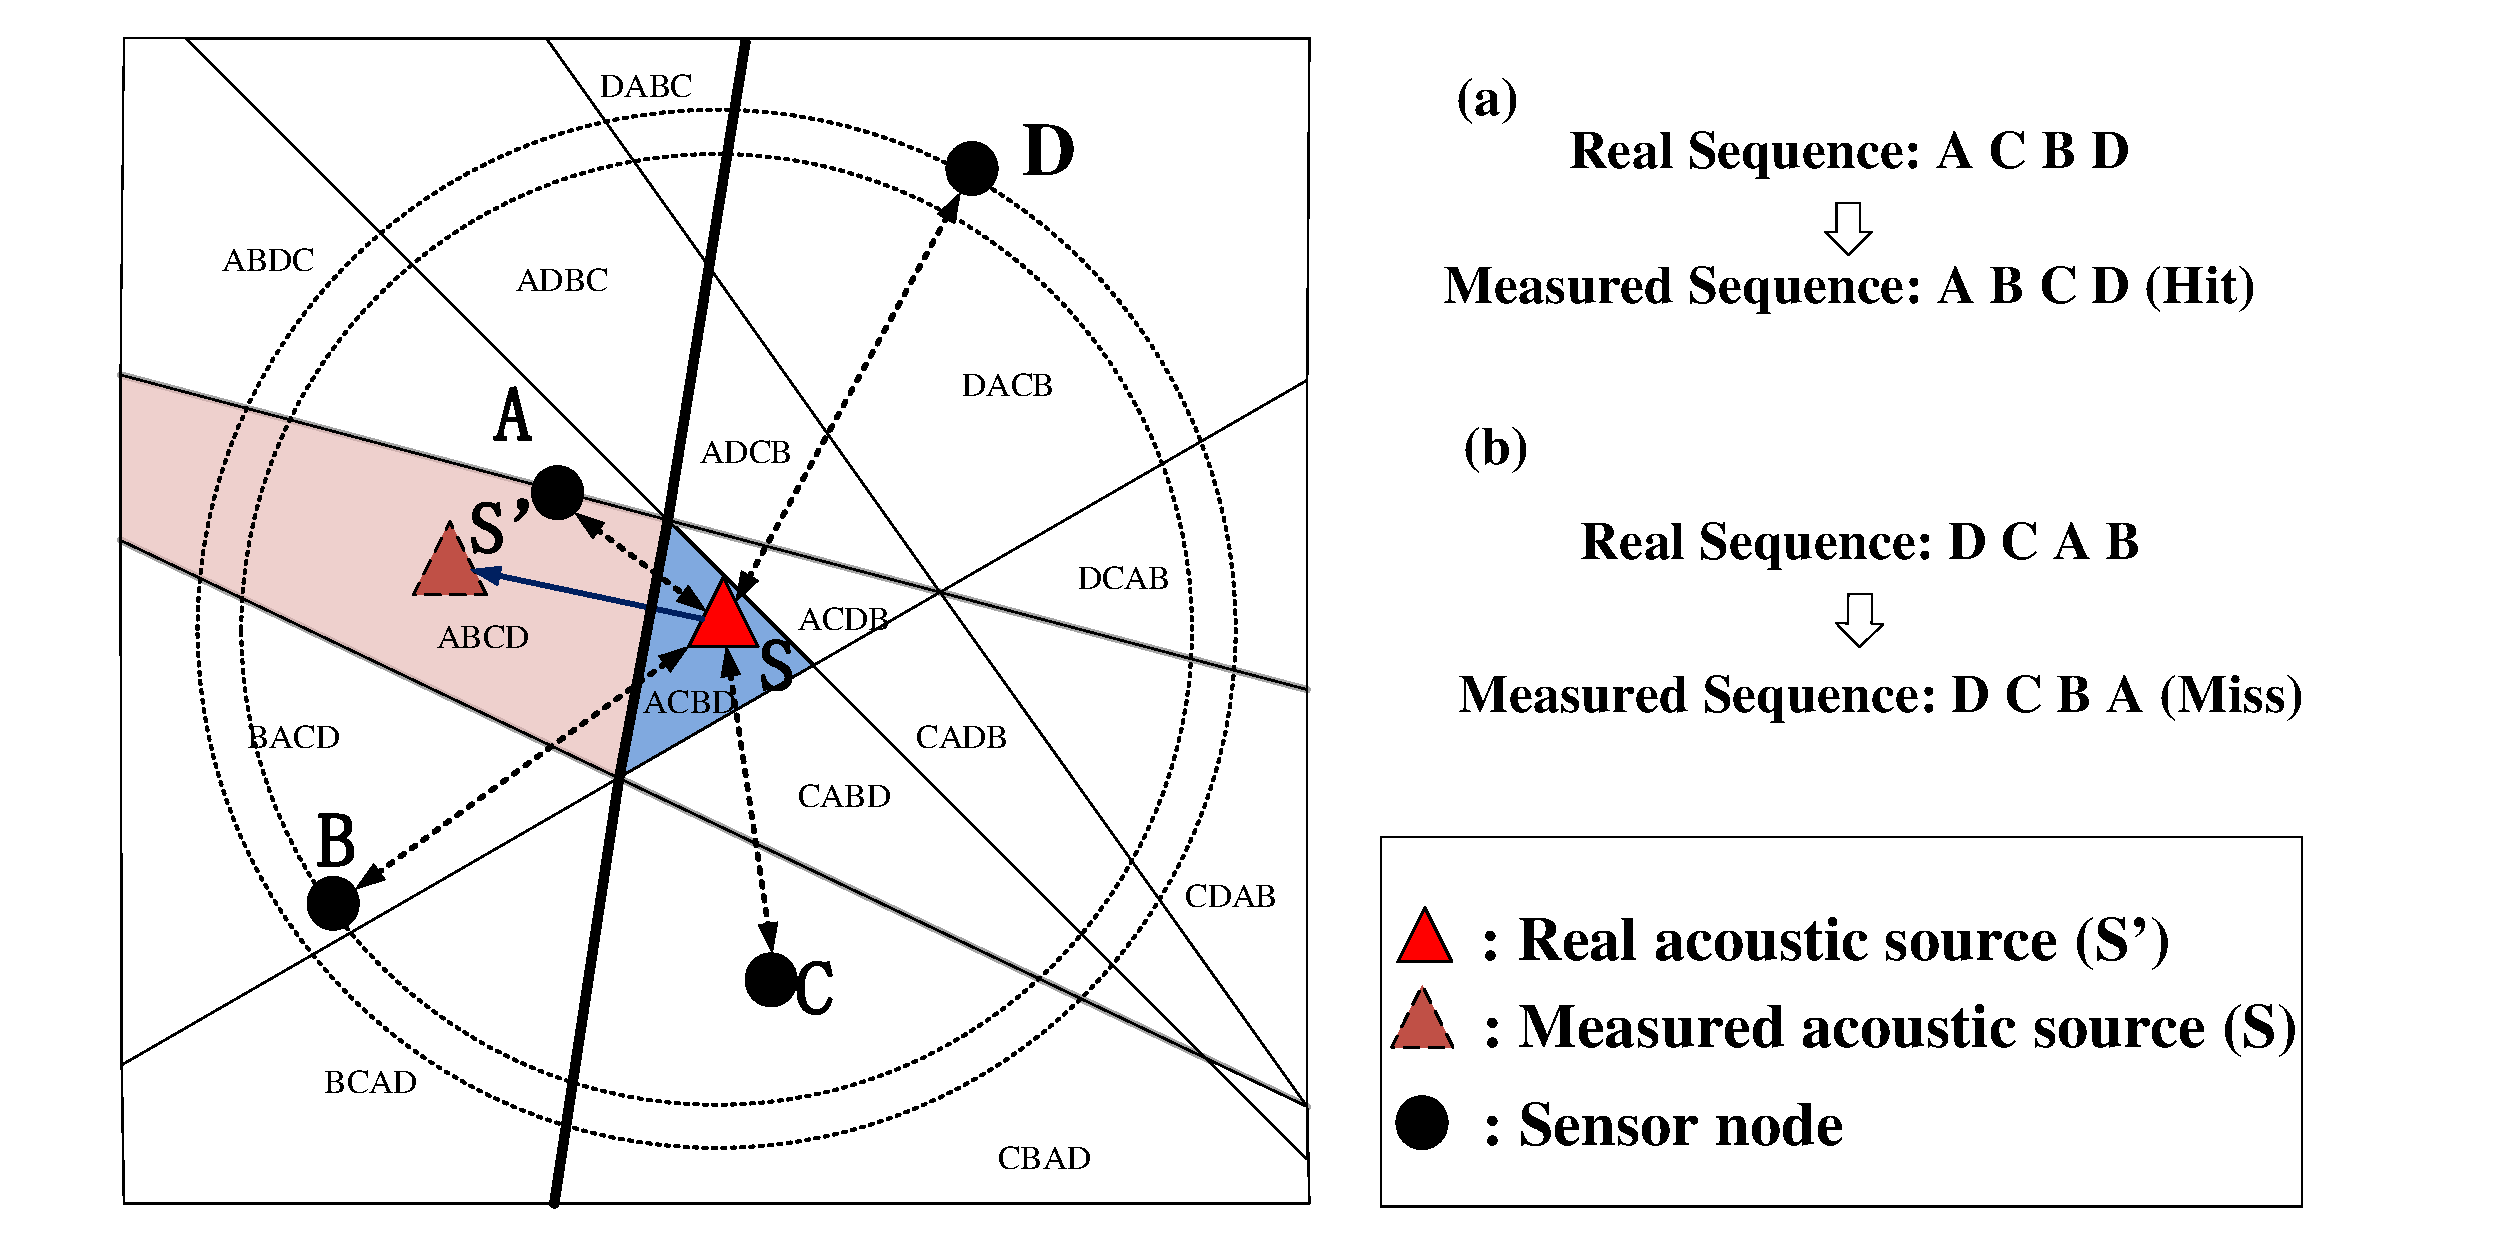
\includegraphics[height=4.5cm]{image/fig2.eps} 
	\vspace{10mm}
    \caption{Flip Tolerance}
	\label{fig2}
    \vspace{-5mm}
    \end{figure}

For the sake of presentation, until now we have described LPSBL in an ideal case where a complete and perfect node sequence can be obtained. 
In this section, we describe how to make LPSBL work well under more realistic conditions. 

In the practical application, if two nodes are located too close to each other along the direction of event propagation, they detect the event almost simultaneously. 
In this case, the node ordering in the sequence may occur flip. 
For instance, the true sequence is $NodeSeq ( \cdots ,i,j, \cdots )$, but the detected sequence is $NodeSeq ( \cdots ,j,i, \cdots )$.
Algorithm 1 can find a solution to this feasibility program only if there is an embedding satisfying all of the constraints. 
However, it is impossible to find a feasible solution that satisfies all of the constraints when sequence flip occurs. 
For example, as showed in Fig. 2, the right middle region identifies by the node sequence $NodeSeq (D C A B)$. 
Once the order of node A and B occur flip in $NodeSeq (D C A B)$, the region corresponding to $NodeSeq (D C B A)$ does not exist, Algorithm 1 can not give the accurate estimation.
In this section, we propose the solution to address the problem of sequence flip using traditional convex relaxation techniques.


We thus introduce a slack variable ${\xi _{ij}}$ for each inequality constraint to allow for inequality violations.
Rewrite the inequality constraint (\ref{equation_2}) as
 \begin{equation} \label{10}
 d_i - d_j  \le  0 ; \  i,j \in S
 \end{equation}
 Relax the inequality constraint (\ref{10}) to
 \begin{equation} \label{11}
 d_i - d_j  \le  \xi _{ij} ; \  i,j \in S
 \end{equation}
 where
 \begin{math}
 \xi _{ij}  > 0
 \end{math}.
 
As a result, LPSBL with error tolerance can be formulated as a convex optimization problem with linear inequalities constraints as follows:
 \begin{equation} \label{5}
\quad \quad \quad \mathop {\min }\limits_{{x_i},{y_i}} \sum\limits_{(i,j) \in X} {{\xi _{ij}}};\  \xi _{ij} \ge 0\\
  \end{equation}
  \begin{align*}
 s.t.\   d_i - d_j  \le  \xi _{ij} \
\end{align*}
where the objective function of optimization problem is the total amount of all slacks. 

In the optimization problem expressed by the equation \eqref{5}, the problem of inequality violations can be solved by introducing a slack variable for each inequality \cite{Boyd2004}.
Therefore, the proposed LPSBL can provide the robust estimation when the problem of sequence flip occurs.






% Sequence flip may provide more constraints to sequence-based localization. 
% When the position of two nodes in the node sequence is often chanced for multiple measurement, it means that the distances from the acoustic source to the two node are nearly common:
  % \begin{equation} \label{12}
% \left\| {SB - SA } \right\| \le \xi _{ij}
 % \end{equation}
% where $\rho$ is given threshold parameter. Inequality \eqref{12} is equivalent to the following two linear constraints

% \begin{eqnarray} \label{13}
% \begin{array}{l}
 % SB-SA \le \xi _{ij}  \\
 % SA-SB \le \xi _{ij}  \\
 % \end{array}
% \end{eqnarray}



% \subsection{Robust LPSBL}

% Considering the uncertainty of the measurement,
% Given the following node sequence $NodeSeq( \cdots ,i,j, \cdots )$, the uncertainty of ${d_i} < {d_j}$ can be described as : 
% \begin{equation}
% p({d_i} < {d_j})>\alpha
% \end{equation}

% Considering the uncertainty of the location of anchor node and the uncertainty of the measurement together, we have
% \begin{equation}
% p((x_i-x_s)^2+(y_i-y_s)^2 < (x_j-x_s)^2+(y_j-y_s)^2)>\alpha
% \end{equation}
% where ${x_i,y_i}$ and ${x_j,y_j}$ are modelled as independent random variables following the normal distribution with the known parameter in the inequality.



\subsection{Incremental LPSBL }

\begin{algorithm}
\caption{Incremental LPSBL Method}
 \KwIn { the first two data package $pack_i$ $pack_j$ \\
 \hspace{0.41in} newest data package $pack_k$ \\
 }
 \KwOut {Location of the acoustic source}
 
 \textbf{Step 1:}  Initial LP problem using the first two data package $pack_i$ $pack_j$ \\
          while (the newest data package $pack_k$ reach)\\		 
		   $pack_k$ ($ID_k$,$Location_k$,$TOA_k$)\\
\textbf{Step 2:}  Constructing inequality constraint according to the TOA of the newest data package : \\ 

\textbf{Step 3:} Solve LP problem to get the target's location.\\
       
 
 \end{algorithm}


\subsection{Complexity Analysis}
This section provides the complexity analysis for the proposed
LPSBL design. It needs to be emphasized that
LPSBL itself adopts an asymmetric design in which sensor
nodes need only to detect and report the events. Therefore,
we only analyze the computational cost on the node sequence
processing side, where resources are plentiful.

SBL: Calculating the Spearman’s coefficient and Kendall’s Tau
between two sequences are $O(N)$ and $O(N^2)$ operations,
respectively. Since the location sequence table is of size
$O(N^4)$, searching through it takes $O(N^5)$ and $O(N^6)$ operations,
respectively~\cite{yedavalli2008sequence}.

LPSBL: The complexity of low dimensional linear programming
with L constraints is $O(L)$\cite{Griva2009}. The number of linear constraints is $N(N-1)/2$ in LPSBL,
where $N$ is the number of nodes. Thus, the overall computation
complexity of LPSBL can be written as $O(N^2)$.




\section{Discussion}

\subsection{multiple measurement}
 Sequence flip may provide more constraints to sequence-based localization. 
 When the position of two nodes in the node sequence is often chanced for multiple measurement, 
it means that the distances from the acoustic source to the two node are nearly common:
   \begin{equation} \label{12}
 \left\| {SB - SA } \right\| \le \xi _{ij}
  \end{equation}
 where $\rho$ is given threshold parameter. Inequality \eqref{12} is equivalent to the following two linear constraints

 \begin{eqnarray} \label{13}
 \begin{array}{l}
 SB-SA \le \xi _{ij}  \\
  SA-SB \le \xi _{ij}  \\
  \end{array}
 \end{eqnarray}



 \subsection{the uncertainty of the measurement}
% Linear Programming with Probability Constraints - Part 1
% Chance Constrained Programming
% Cutting-plane
%k-Violation linear programming
 Considering the uncertainty of the measurement,
 Given the following node sequence $NodeSeq( \cdots ,i,j, \cdots )$, the uncertainty of ${d_i} < {d_j}$ can be described as : 
 \begin{equation}
 p({d_i} < {d_j})>\alpha
 \end{equation}

  \subsection{the uncertainty of the location of anchor node}
 Considering the uncertainty of the location of anchor node and the uncertainty of the measurement together, we have
 \begin{equation}
 p((x_i-x_s)^2+(y_i-y_s)^2 < (x_j-x_s)^2+(y_j-y_s)^2)>\alpha
 \end{equation}
 where ${x_i,y_i}$ and ${x_j,y_j}$ are modelled as independent random variables following the normal distribution with the known parameter in the inequality.




\subsection{Time Synchronization }

Like the effect of TOA detection error, time synchronization error maybe also occur flip problem when computing the node sequence in LPSBL system, then lead to localization error.
Traditional time synchronization protocol, such as RBS, TPSN, and FTSP, can achieve synchronization less than 100ns. 
Compared with the the measurement error of TOA, time synchronization error has little effect on the LPSBL system.

% \subsection{Multiple Source Localization}

% Localizing multiple, simultaneously active sources is a more difficult problem. 
% In order to avoid conflict of several source, multiple source localization must be able to uniquely identify the signature of each acoustic source, which is beyond the capability of this paper. 
% So we will not do too much discussion about it in this paper.
% We just take an example, if the several targets are set as shown in Fig. 3, then we can calculate the location of the targets 
% because the acoustic source I is far enough from source II and the single from them can be distinguished. 
% So the smartphones close to the area I could handle the source I, and another smartphones close to the area II could handle the source II. 
% The Fig. 3 also describes system scalability.
% We can use a range to divide the large-scale area into to a smaller area that is large enough to cover the coverage of the acoustic source's signal.
% And the small area can be handled as our algorithm proposed by preceding part of the paper.

% %  \label必须放在\caption命令的后面
  % \begin{figure}[ht]
            % \setlength{\abovecaptionskip}{0pt}
            % \centering
            % 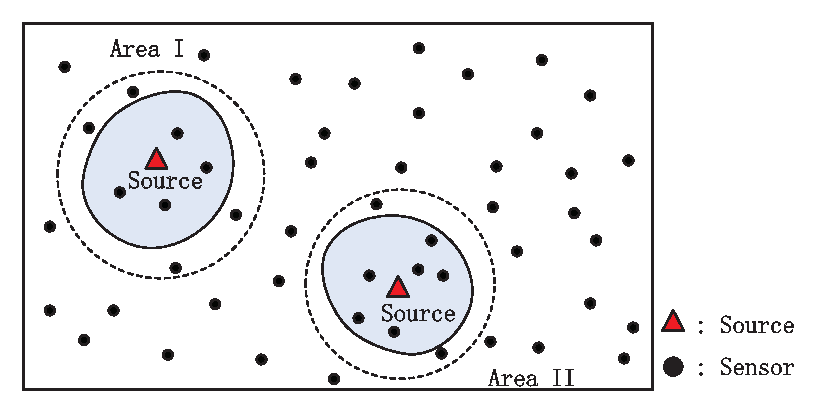
\includegraphics[scale=1.4,height=4.0cm]{image/fig3.eps}
             % \vspace{1mm}
			% \caption{Scalability for large-scale system}
			% \label{Fig3}
            % \label{multiple_source_localization}
            % \vspace{-5mm}
  % \end{figure}


% \subsection{Energy Efficiency}
% Energy efficiency is another issue in distributed acoustic sensor networks.
% Most of the time, acoustic sensor nodes keep asleep until the acoustic source appears in its sensing area.  
% The smartphone nodes near the acoustic source detect the acoustic signal, then alert its neighbour smartphones to prepare for receiving the signal.
% In this way, the proposed LPSBL system can save energy of acoustic sensors, then prolong the service life of distributed acoustic sensor networks.








\section{EVALUATION }
\label{section:results}

\subsection{Simulation}
In this section, we try to simulate our sequence-based localization technique based on linear programming (LPSBL) with SBL method using MATLAB. 
In the simulation, we randomly generate a lot of smartphones in a $10m \times 10m$ area. 
Considering the impact of the uncertainty of node position and TOA detection, we add a certain amount of node location error and TOA measure error in all the simulations.
All the statistics are running more than 100 times for high confidence, and reported by RMSE figure. Table 1 illustrates the default simulation setup parameters.

\begin{table} \normalsize
\caption {\textbf{Default configuration parameter}} %title of the table
\centering % centering table
    \begin{tabular}{|c|c|}
        \hline
Parameter & Description \\
 \hline
Field Area & 10m $\times$ 10m \\
\hline
Number of Anchors & 50 (Default) \\
 \hline
Node Location Error 	 & 0.10m (Default) \\
 \hline
TOA Detection Error 	 & 0.10ms (Default) \\
 \hline
Random-Seed Loop	 & 500 times (Default) \\
 \hline
Error Statistics	 &  RMSE \\
        \hline
    \end{tabular}
\end{table}



The results of simulation evaluation are as following:


\textbf{1) Impact of the number of anchors:}
 In this experiment, we investigate the localization error and number of anchors with a different number of anchors from 10 to 40 in steps of 2. 
 We run the simulation with the TOA error is 0.1ms, and other simulation parameters are default. 
 Since the two localization methods being compared are aiming to locate the target by processing the anchors, 
 but the SBL method can cause a big error, while the LPSBL method is aiming to avoid the appearance and get better result. 
 We can speculate that with more anchors, the whole area will be divided into smaller parts, 
 thus more accurate localization estimation should be achieved in the LPSBL method. 
Fig. \ref{fig4} confirms our expectation. As shown in Fig. \ref{fig4}, with the number of anchors increases, localization error for both  methods are down slowly. 
Fig. \ref{fig4} also shows that the localization error of the LPSBL method is approximate to the SBL method when the number of anchor node is larger.
  \begin{figure}[htb]
            \setlength{\abovecaptionskip}{0pt}
           % \centering
			 \vspace{-15mm}
           		 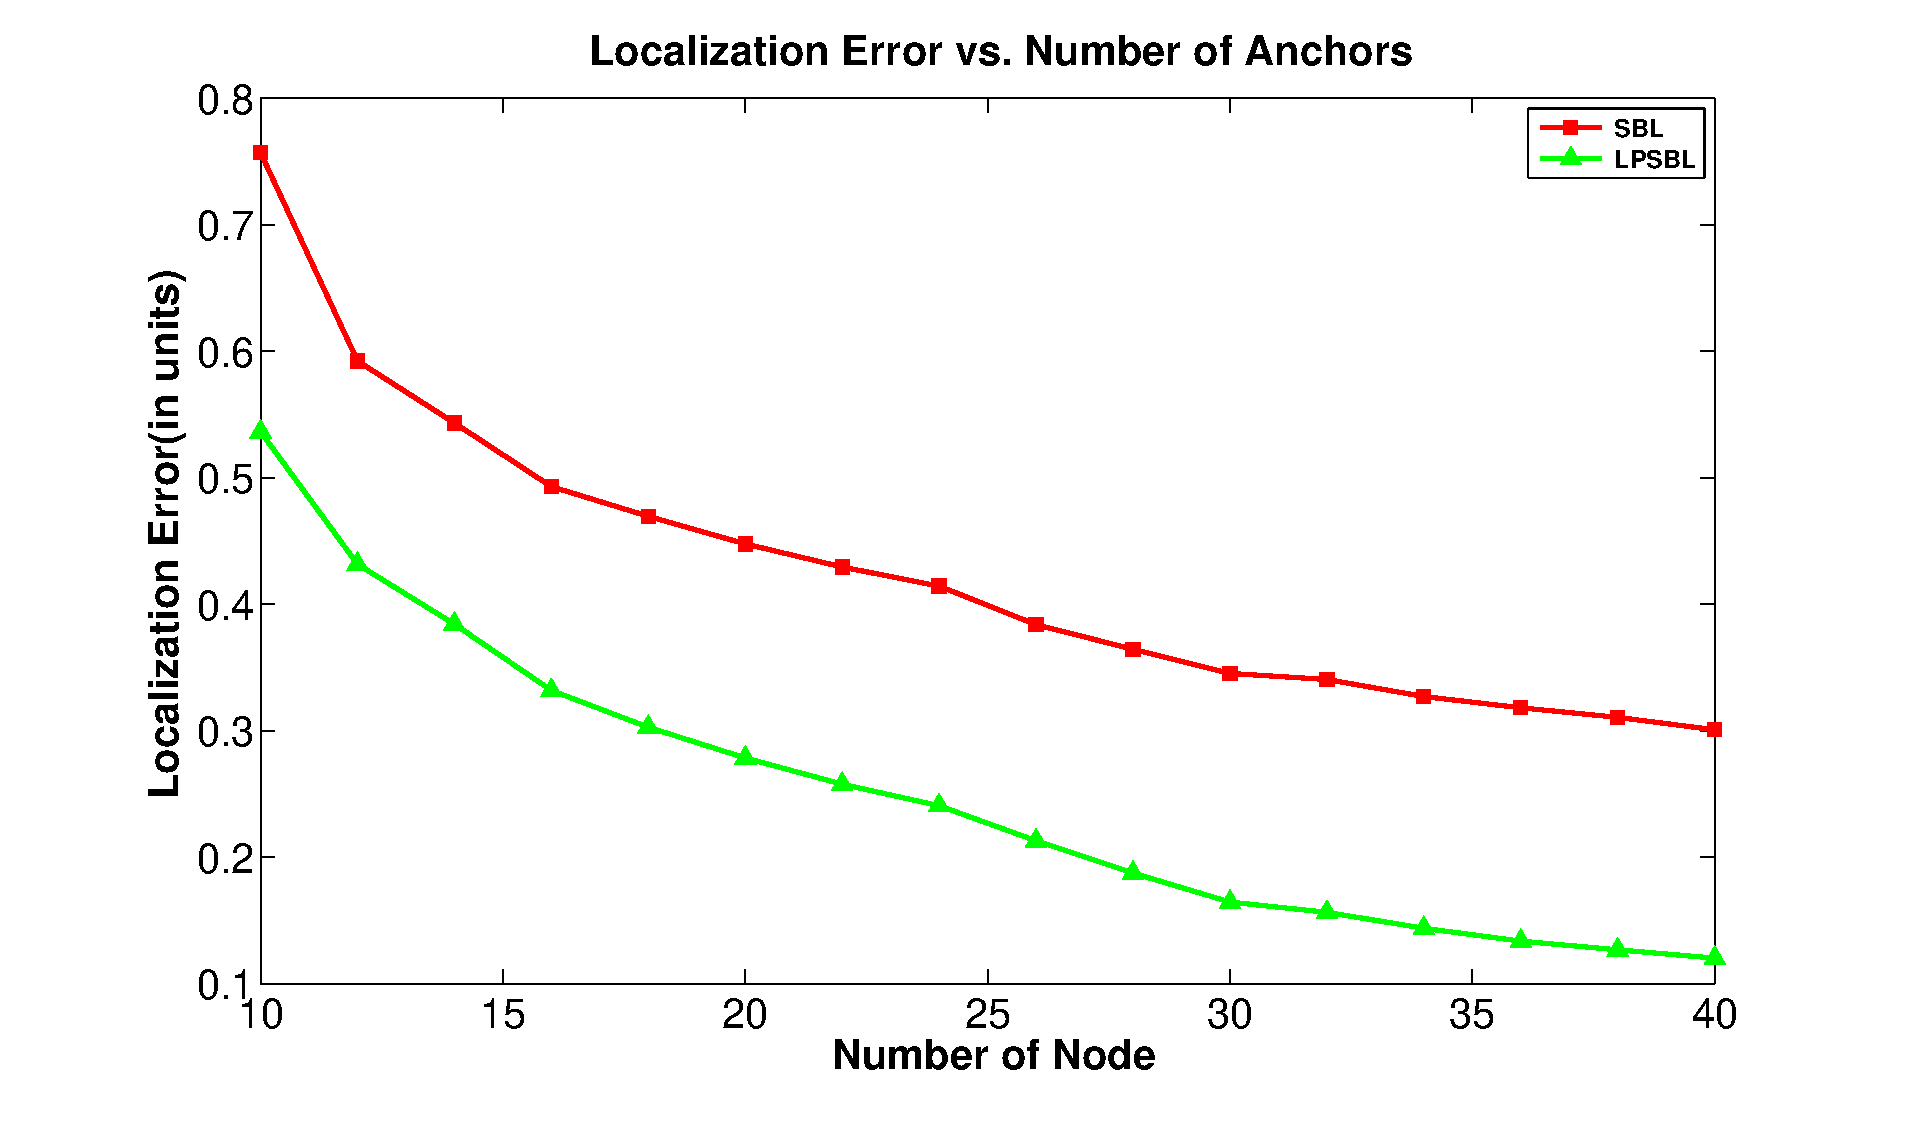
\includegraphics[height=5.0cm,width=7.0cm]{image/fig4.eps}
            \vspace{15mm}
            \caption{Localization Error vs. Number of Anchors}
             \vspace{-5mm}
             \label{fig4}
        \end{figure}	
		
\textbf{2) Impact of the location error:}
 In this experiment, we compare the two methods for different location errors of anchors. 
 In Fig. \ref{fig5}, we choose the location error with the range from 0 to 0.4m in step of 0.02m for the two methods. 
 Fig. \ref{fig5} indicates the location error of anchors has an effect on the positioning results. 
 The proposed LPSBL method are more accurate than the SBL method. 
 For the SBL method, the positioning error changes obviously as location error increases in Fig. \ref{fig5}. 
 However, as demonstrated in Fig. \ref{fig5}, the positioning error of LPSBL varies little, which demonstrates the LPSBL method is the most robust to the node location error.
  \begin{figure}[htb]
          %  \centering
		   \vspace{-25mm}
			 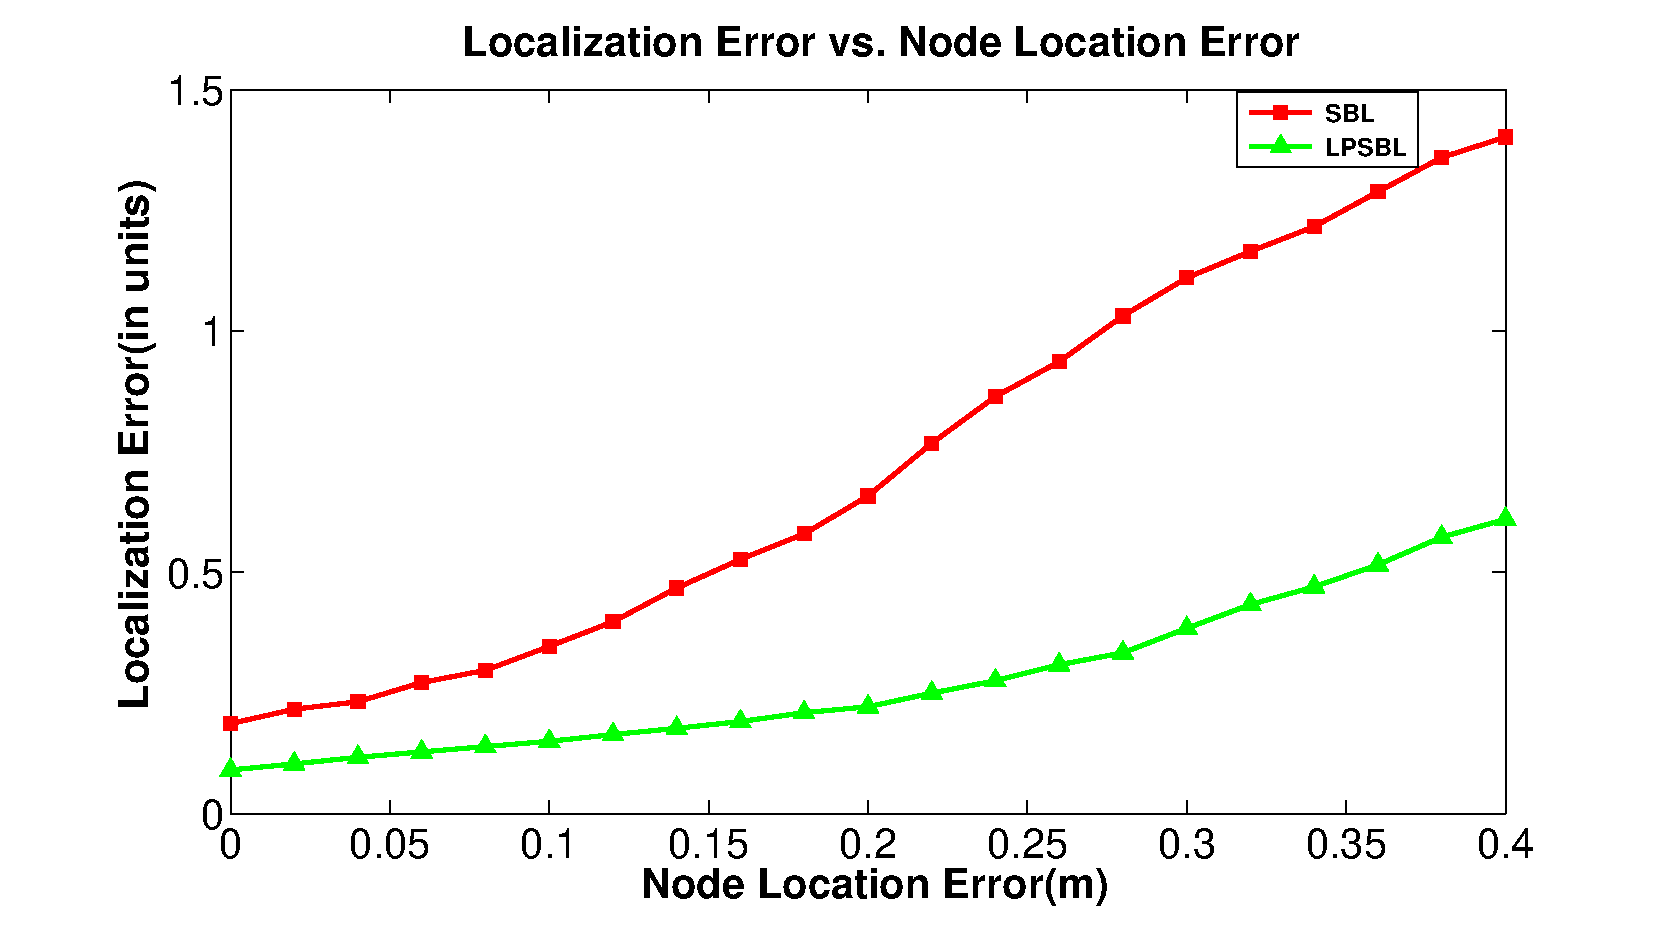
\includegraphics[height=5.0cm,width=7.0cm]{image/fig5.eps}
            \vspace{25mm}
            \caption{Localization Error vs. Node Location Error}
             \vspace{-5mm}
             \label{fig5}
        \end{figure}

\textbf{3) Impact of the TOA measurement error:}
In this experiment, we perform the impact of the TOA error of anchors for the two methods being compared with the range from 0 to 2ms in steps of 0.1ms. 
Other simulation parameters keep default. 
We can guess that the TOA measurement error may influence the localization accuracy. 
Fig. \ref{fig6} confirms it. As it is shown in Fig. \ref{fig6}, the localization error of the  two methods is increasing as the TOA error growth. 
Thus, we can determine the speculation that the error of TOA measurement can influence the localization accuracy is true. 
Also, the LPSBL method has a better result than the SBL method. 
%The Robust LPSBL method get the best experimental result. 
It is shown in Fig. \ref{fig6}, the localization error of our LPSBL method is stable no matter which degree the TOA error is, which means that the LPSBL method can localize the target node with little error when TOA error is not too big.
  \begin{figure}[htb]       
           % \centering
			\vspace{-15mm}
            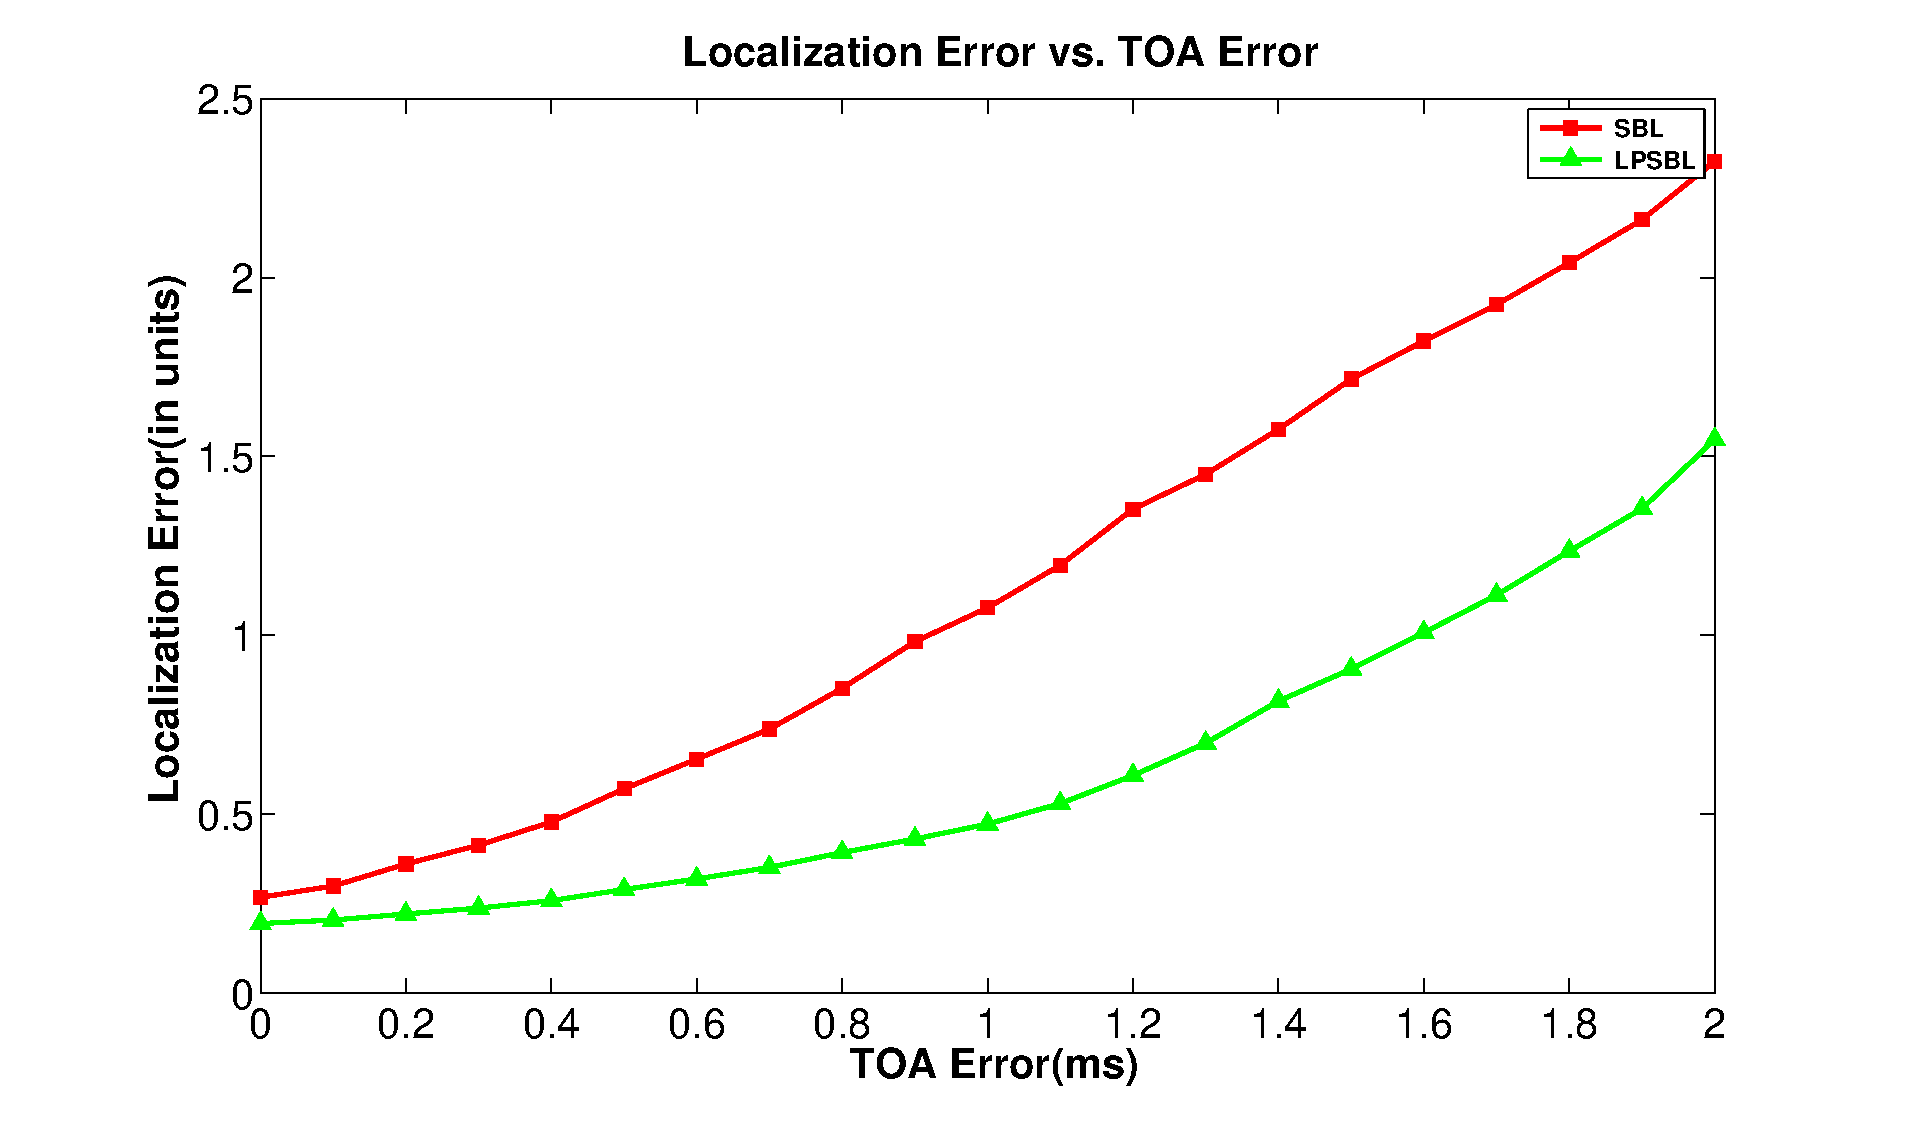
\includegraphics[height=5.0cm,width=7.0cm]{image/fig6.eps}
           \vspace{15mm}
            \caption{Localization Error vs. TOA Error}
             \vspace{-5mm}
             \label{fig6}
        \end{figure}
		
 \textbf{Summary:} From the above simulations, considering the different factors, including the number of anchors, the node location error and TOA measurement error of the anchors, we can get the following conclusions:

 (1) With increasing number of the number of anchors, localization errors decrease for both methods, and LPSBL has better localization performance;

 (2) The error of node location can impact the localization error, the proposed LPSBL method is more robust to the error of node location than SBL method;
 
 (3) The TOA measurement error has a major impact on the localization accuracy, and the proposed LPSBL method can achieve better localization performance.



\subsection{Emulation}


In this section, we report system implementation of our design based on smartphones.
we use 30 Samsung smartphones as anchors and connect them through CISCO CVR328W-K9-CN wireless router. 
TPSN protocol is adapted in the proposed LPSBL system to realize time synchronization.
The 30 smartphones are deployed in a size of 16m$\times$10m space and there just one target during an experiment.
In the experiment, smartphones are random deployed in the space, and 100 times localization results are showed in Fig.~\ref{fig7}. 
In the figure, blue squares stand for anchor
nodes, red circle squares are the real position of acoustic sources, and black dot are the estimated location by LPSBL. 
An arrow origins from the estimated location of each acoustic source and points to its real position. 
As the results showed in Fig.\ref{fig7}, most of estimated locations are close to the ground truth and the errors between them are very small,
which means that LPSBL can effectively localize the acoustic source with good robustness.
  \begin{figure}[htb]
              %    \centering
			    \vspace{-12mm}
            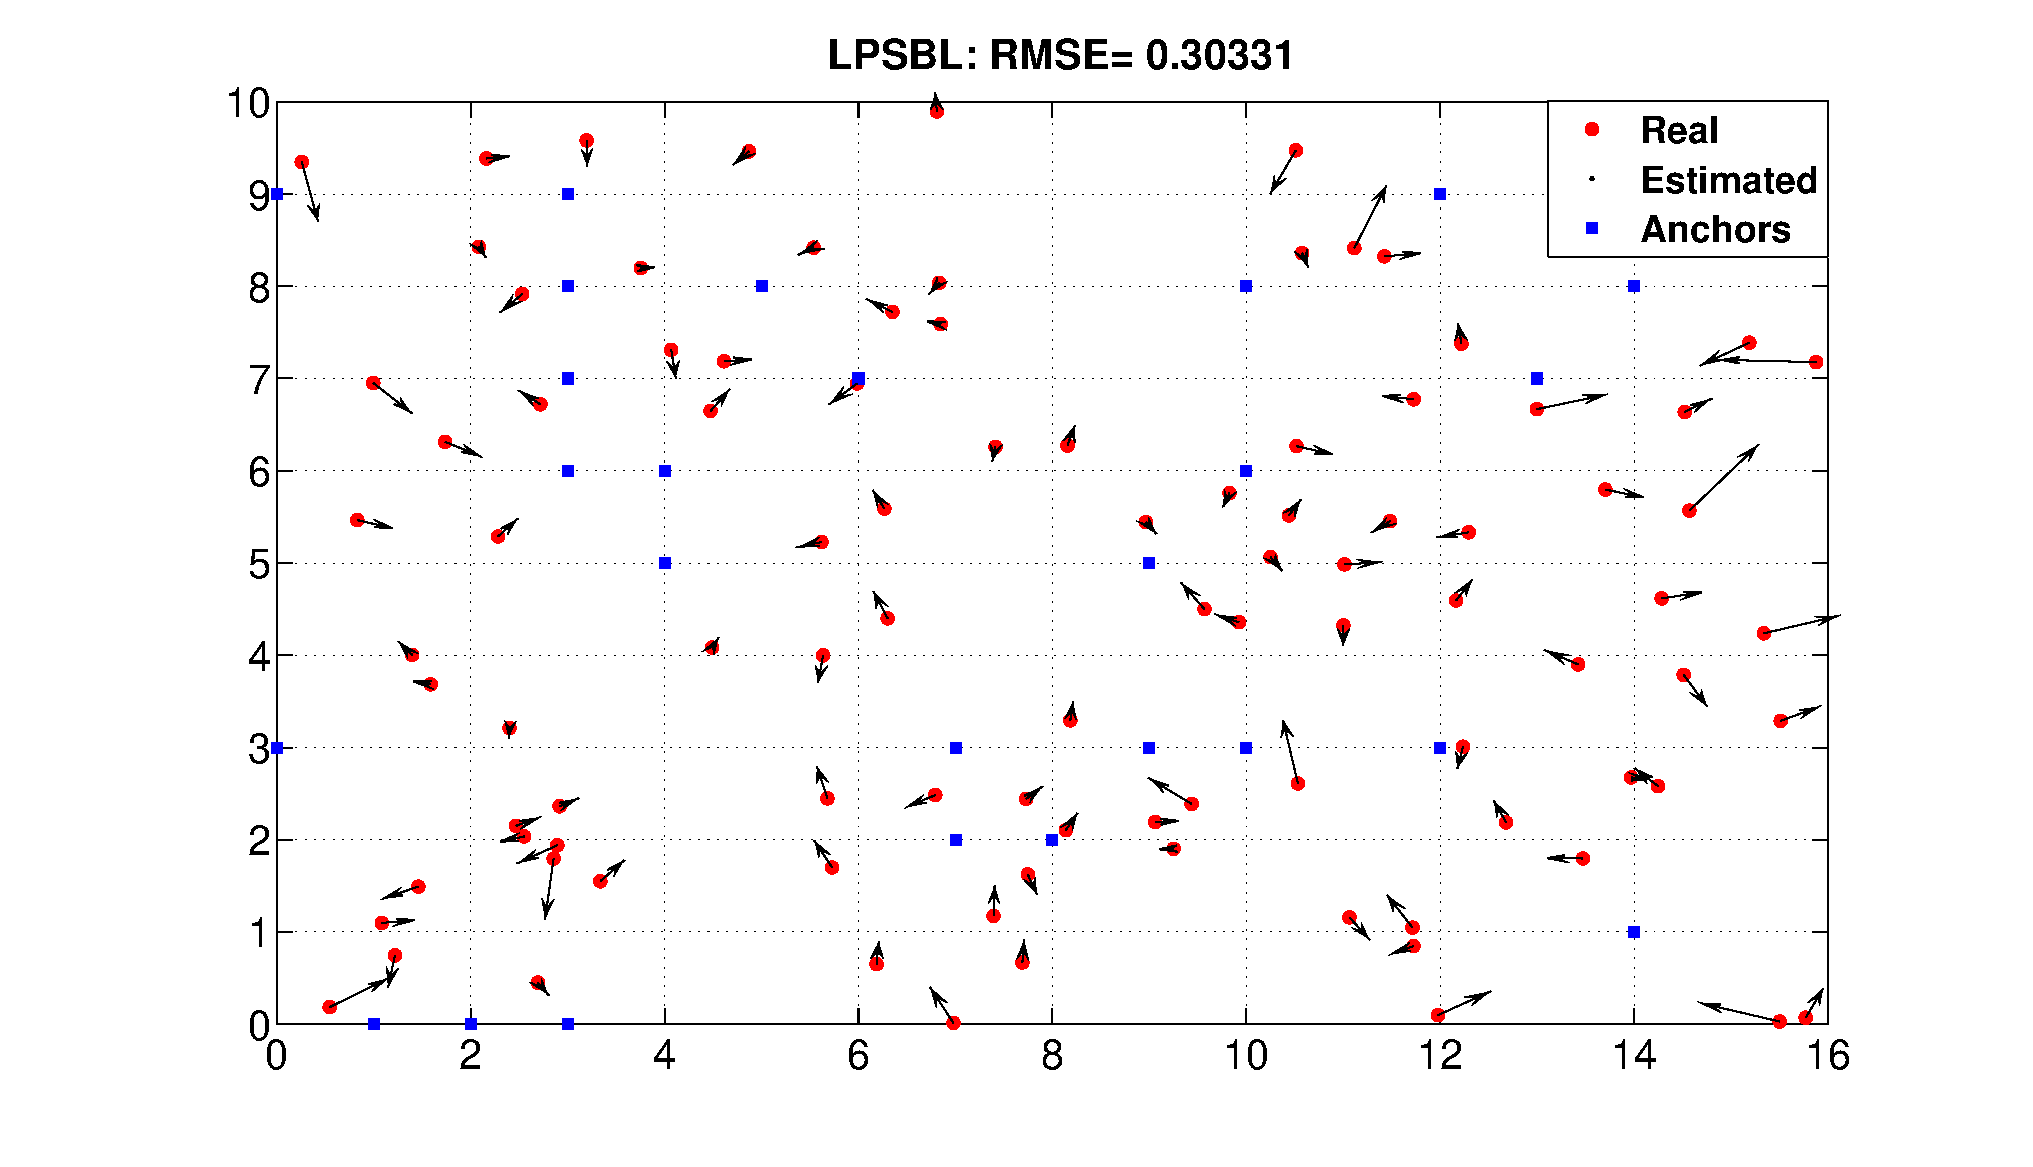
\includegraphics[height=5.0cm,width=7.0cm]{image/fig7.eps}
            \vspace{12mm}
            \caption{Test-bed localization result of the proposed LPSBL}
             \vspace{-5mm}
             \label{fig7}
        \end{figure}

\section{Related Work}

Acoustic source localization in sensor network is a widely-studied problem. 
In the past few years, there has been a growing interest for spatial distributions of independent (unsynchronized) acoustic sensors, each made of two or more synchronized microphones. Due to space constraints, we can only mention a few directly related works here.
% Omologo, \emph{et al.} \cite{omologo1994acoustic} compute the Steered Response Power maps associated to all the microphone pairs over a spatial grid and then localize the source
% as the peak of the cumulative global map, with overall computational costs that are often too demanding for the application at hand.
% Better computational efficiency is achieved in \cite{cobos2011modified} where the SRP  accommodates a different computation over a coarser grid.
% Alternate approaches based on Least Squares were proposed in \cite{rabinkin1996dsp} with a certain sensitivity to environmental noise;
% and in \cite{do2007real} where a stochastic region contraction of the grid was proposed, adopting a multi-resolution approach.
Wang, \emph{et al.} \cite{wang2003acoustic} described a system having static cluster architecture, the system experienced a problem in that the accuracy decreased when an acoustic source occurred between the clusters.
Chen, \emph{et al.} \cite{chen2004dynamic} showed that nodes in the system did not need to recognize their cluster head, reducing the constraints on deployment of the localization system.
Hu, \emph{et al.} \cite{hu2009design} design the system based on 2-tier architecture, which experienced cost and deployment problems especially in the very large target area.
Rabbat, \emph{et al.} \cite{rabbat2005robust} proposed a decentralized algorithm based on the distributed ML estimation technique using token ring architecture.
Kim, \emph{et al.} \cite{kim2009locating} proposed to identify the node closest to the acoustic source, based on TOA comparisons between all nodes, thus incurring high communication cost and requiring global synchronization between all sensor nodes.
Lightning is a method proposed in \cite{wang2008lightning} to identify the sensor closest to the acoustic source, also based on expensive broadcasting/flooding.
In previous research on distributed acoustic source localization system, generally each node just has a single element. 
In the past few years, there has been a growing interest for acoustic nodes made of two or more synchronized microphones. 
Aarabi, \emph{et al.} ~\cite{aarabi1900fusion} used 10 dual-microphone arrays distributed in a room and used their data to locate three speakers.
Wu, \emph{et al.} ~\cite{wu2012fusion} used three dual-microphone arrays to locate two sound sources in a distributed way in which only the local DOA estimates are communicated among arrays.
Canclini, \emph{et al.}\cite{canclini2013acoustic,Canclini2015} proposed a method for localizing an acoustic source with distributed microphone networks based on TDOA between microphones of the same sensor.

Most of the existing acoustic source localization methods in sensor networks are based on range-based measurement.
In contrast, our work is a range-free method and shown to be robust to the errors of node locations and the errors of measurements.
There have existed some research on range-free localization method.
Yedavalli, \emph{et al.} ~\cite{yedavalli2008sequence} proposed a Sequence-Based Localization (SBL) method in WSN. 
The heart of SBL is the division of a 2D localization space into distinct regions by the perpendicular bisectors of lines joining pairs of reference nodes (nodes with known locations).
%Each distinct region formed in this manner can be uniquely identified by a location sequence that represents the distance ranks of reference nodes to that region. 
%The unknown node first determines its own location sequence based on the measurement between itself and the reference nodes, then searches through the location sequence table to determine its location.
In their earlier work \cite{yedavalli2005ecolocation}, Ecolocation used location constraints for robust localization.
%A location constraint is a relationship between the distances of two reference nodes from the unknown node that determines its proximity to either
%reference nodes. Location constraints can be graphically represented by perpendicular bisectors
%between reference nodes, and each location sequence can be written as a set of location constraints.
%Thus, the location constraint set is also unique to each region in the arrangement.
Chakrabarty, \emph{et al.} \cite{chakrabarty2002grid} and Ray, \emph{et al.} \cite{ray2004robust} use identity codes to determine the location of sensor nodes in grid and nongrid sensor fields, respectively. 
% Here, each grid point or region in the localization space is identified by a unique set of reference node IDs whose signals can reach
% the point or region, and this unique set is an identity code for that point or region. 
e, \emph{et al.} \cite{he2003range} propose an RF-based localization technique in which the unknown node location is determined by the intersection of all triangles,
formed by reference nodes, that are likely to bound it. The unknown node determines its existence inside a triangle by
comparing its measured RSS values to that of its neighbors to detect a trend in RSS values in any particular direction
This technique depends on the weak assumption that signal strength decreases monotonically with distance, which is not true in real-world scenarios.
Zhong, \emph{et al.} \cite{zhong2009tracking} convert the original tracking problem to the problem of finding the shortest path in a graph, which is equivalent to optimal matching of a series of node sequences. 
Zhong, \emph{et al.} \cite{zhong2011rsd} introduce a proximity metric called RSD to capture the distance relationships among 1-hop neighboring nodes in a range-free manner. 
Guo, \emph{et al.} \cite{guo2014detecting}  proposed a novel method to detect nodes with data faults by ranking the nodes based on their sensing
readings from the event.
Shu, \emph{et al.} \cite{shu2015toc}  proposed a novel localization design that utilizes the unique Time of Charge (TOC) sequences among wireless rechargeable sensors.
Zhong, \emph{et al.} \cite{zhong2012wireless} presented a Multi-Sequence Positioning (MSP) method for  sensor node localization by processing multiple one-dimensional node sequences.
Yang, \emph{et al.} \cite{yang2013freeloc} use the relative relationship information between RSS values as the fingerprint data in the Wi-Fi indoor positioning system.


%localize nodes based on their connectivity information or simple sensing of their relative positions.

%rang free ??
%Q. Xu, A. Gerber, Z. M. Mao, and J. Pang. 2011. AccuLoc: Practical localization of performance measurements in 3g networks. In ACM MobiSys.

%rang free ?? L. Doherty, K. S. J. Pister, and L. El Ghaoui. 2001. Convex position estimation in wireless sensor networks.In IEEE INFOCOM.

\section{Conclusions}

In this paper, we presented a simple and novel node sequence-based localization technique based on linear programming, LPSBL. 
In LPSBL, node sequences are used to uniquely identify distinct regions in the localization space. 
The reference node sequence is computed by using TOA measurements of acoustic signals between the acoustic source and the reference nodes.
The inequality constraint is constructed by processing the nodes sequence, then turn the sequence-based localization into linear programming problem. 
Since our system runs on COTS smartphones and supports spontaneous setup, 
 it has potential to enable a wide range of distributed acoustic source localization systems. 
 Besides the basic design, advanced LPSBL is proposed for further enhancing system robustness.
 Our system is verified and evaluated through analysis, extensive simulation as well as the test-bed experimentation.
 The test results have shown that the proposed method can effectively implement aoustic source localization with ad-hoc smartphone array.
% Our next step is to study the distributed localization method for ad-hoc smartphone array.
% Another future work is that further mining the information embedded in the node sequence to improve the robustness of localization system.

\section*{Acknowledgments}
This work is supported by the Fundamental Research Funds for the Central Universities (Grants No. DUT15QY05, DUT15QY51, No. DUT14ZD218 and DUT14QY29) and is partly supported by Natural Science Foundation of China (Grant No. 61272524).  Naigao Jin is the corresponding author.




\bibliographystyle{IEEEtran}
\bibliography{Main}

\end{document}
